\chapter{Results}
\label{chap:results}

\section{Highly Efficient Image Preprocessing}
The latency of the preprocessing kernel, as discussed in Chapter \ref{chap:debayer}, was measured to be $1.13ms$ using the \code{nsys profile} command line tool from the CUDA toolkit. The kernel is launched with only two thread blocks, which means that we are utilizing a maximum of two out of the eight available \glspl{sm} on the \gls{gpu} \cite{rigerunNVIDIAJetsonXavier2023}. Considering a frame rate of 2$\times$16 frames per second, it indicates that less than $1\%$ of the \gls{gpu} is being utilized for preprocessing purposes.

\begin{equation}
    \frac{2 \times 16 \text{f}/s}{1 \text{f} / 1.13ms} \times \frac{2 \text{SM}}{8 \text{SM}} = 0.904\%
\end{equation}


This estimation is consistent with the observation of $0\%$ \gls{gpu} utilization reported by \gls{jtop} for most of the time. In comparison to the initial implementation using \gls{opencv} on the CPU, where all CPU cores were running at maximum frequency but unable to achieve 32 frames per second, the \gls{gpu} implementation shows a substantial improvement. The benefits of this approach include reduced power consumption and increased availability of both CPU and \gls{gpu} resources for other tasks.

\section{Compression}
The implementation of a compression pipeline in \gls{gstreamer} enables longer recording times and the ability to stream compressed images to the graphical user interface.

During the \master, funding was obtained to upgrade the \jx to a \jo platform.
One notable difference between these two platforms is that the \jo supports \gls{av1} encoding, in addition to all the encoding formats supported by the \jx \cite{karumbunathanNVIDIAJetsonAGX2022}.
Due to the higher efficiency of \gls{av1} compared to \gls{h265}, it was decided not to spend significant time fine-tuning the compression parameters for \gls{h265}, but rather focus on extensive performance testing \cite{torresAV1VsHEVC2022}.
Nonetheless, a brief test was conducted to provide a rough estimate of the expected compression performance of the \gls{h265} encoder.

To measure the compression ratio and error, a test video was recorded while walking around the boat yard area at Nyhavna, capturing the same areas depicted in Figure \ref{fig:picture_1984} and \ref{fig:picture_1536}.
Only one camera was enabled during the recording to be able to write the raw data to disk fast enough.
Utilizing the encoding parameters listed in Table \ref{tab:encoder_parameters}, a compression ratio of almost $4/1$ was achieved, with an average relative error of less than $0.6\%$ and a maximum relative error below $9\%$.

It is important to note that these encoding parameters were not fine-tuned, and the results may not necessarily be representative of the performance that can be achieved with \gls{h265}.
Further testing is scheduled as part of the migration to the \jo platform.
\begin{table}[H]
    \begin{minipage}[b]{.5\linewidth}
        \centering
        \small
        \begin{tabular}{|c|c|}
            \hline
            \textbf{Parameter} & \textbf{Value} \\
            \hline
            preset-level       & 0              \\
            ratecontrol-enable & 0              \\
            profile            & Main10         \\
            control-rate       & 0              \\
            maxperf-enable     & 1              \\
            qp-range           & 0,1:0,1:0,1    \\
            \hline
        \end{tabular}
    \end{minipage}
    \begin{minipage}[b]{.5\linewidth}
        \centering
        \small
        \begin{tabular}{|c|c|}
            \hline
            \textbf{Parameter} & \textbf{Value} \\
            \hline
            quant-i-frames     & 0              \\
            quant-p-frames     & 0              \\
            quant-b-frames     & 0              \\
            iframeinterval     & 16             \\
            num-Ref-Frames     & 8              \\
            num-B-Frames       & 1              \\
            \hline
        \end{tabular}
    \end{minipage}
    \caption{Encoder parameters used for testing.}
    \label{tab:encoder_parameters}
\end{table}

\section{Captured images}
16 fps 10 bit synchonized stereo images!

\begin{figure}[H]
    \centering
    \subcaptionbox{Mean image.\label{fig:normal_img_1536}}{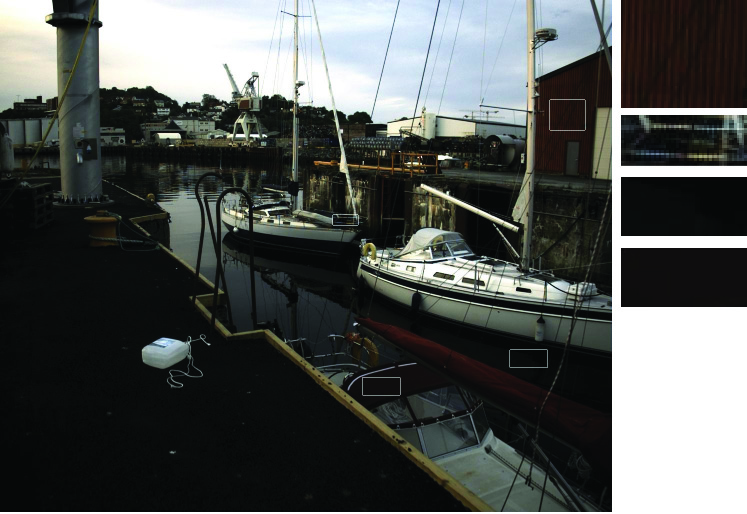
\includegraphics[width=\textwidth]{figures/pictures/result_rgb.jpg}}
    \subcaptionbox{HSV visualization of polarization data where the angle of polarization is encoded as hue and degree of polarization is encoded as value.}{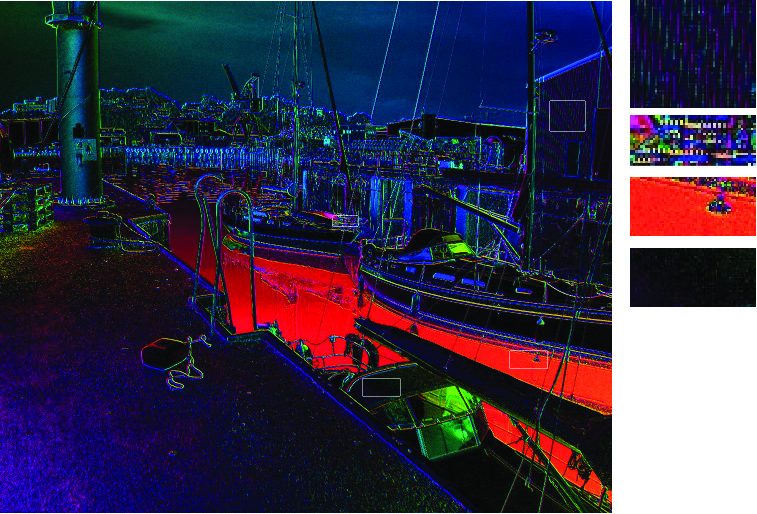
\includegraphics[width=\textwidth]{figures/pictures/result_pol.jpg}}
    \caption{Right image \#1536 with, zoomed in regions of interest.}
    \label{fig:picture_1536}
\end{figure}

\begin{figure}[H]
    \centering
    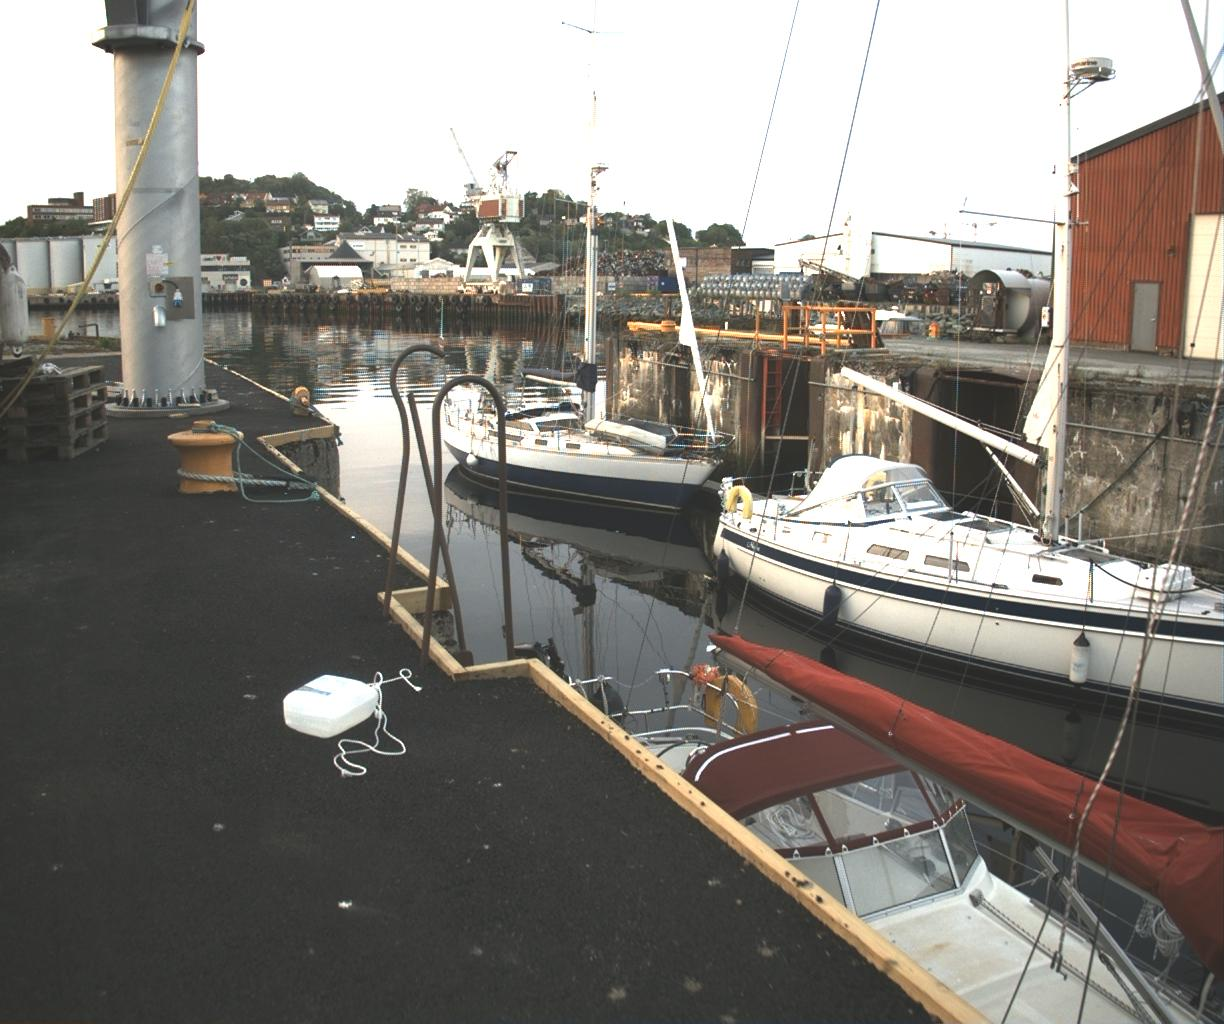
\includegraphics[width=.8\textwidth]{figures/pictures/gained_right_96.jpeg}
    \caption{Image showing how dark areas contain a lot of information thanks to 10-bit depth.
        The image is the same as in Figure \ref{fig:normal_img}, but with brightness increased.}
    \label{fig:gained_image}
\end{figure}

\begin{figure}[H]
    \centering
    \subcaptionbox{Mean image.}{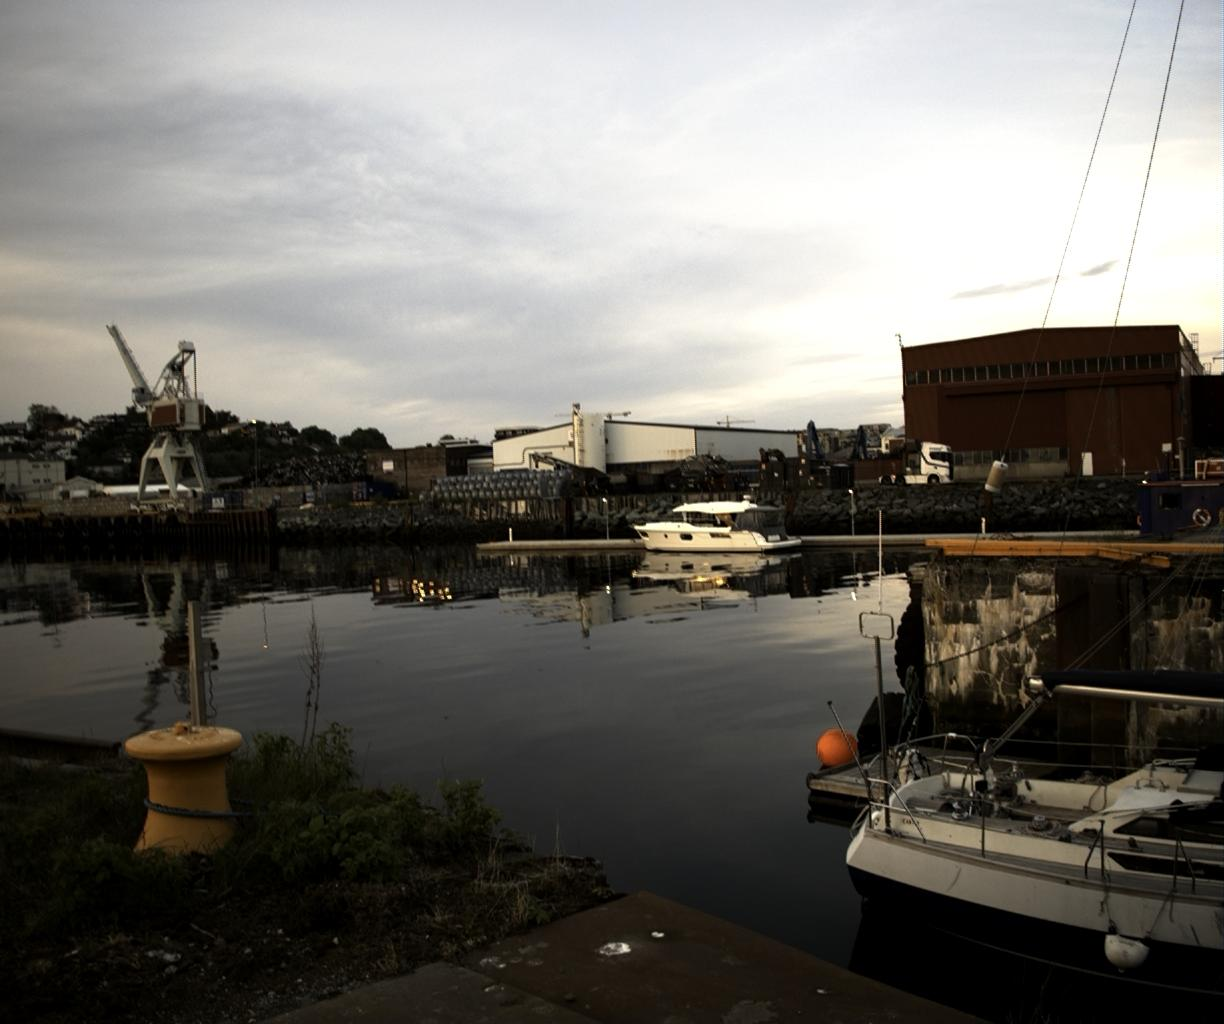
\includegraphics[width=.9\textwidth]{figures/pictures/regular_left_124.jpeg}}
    \subcaptionbox{HSV visualization.}{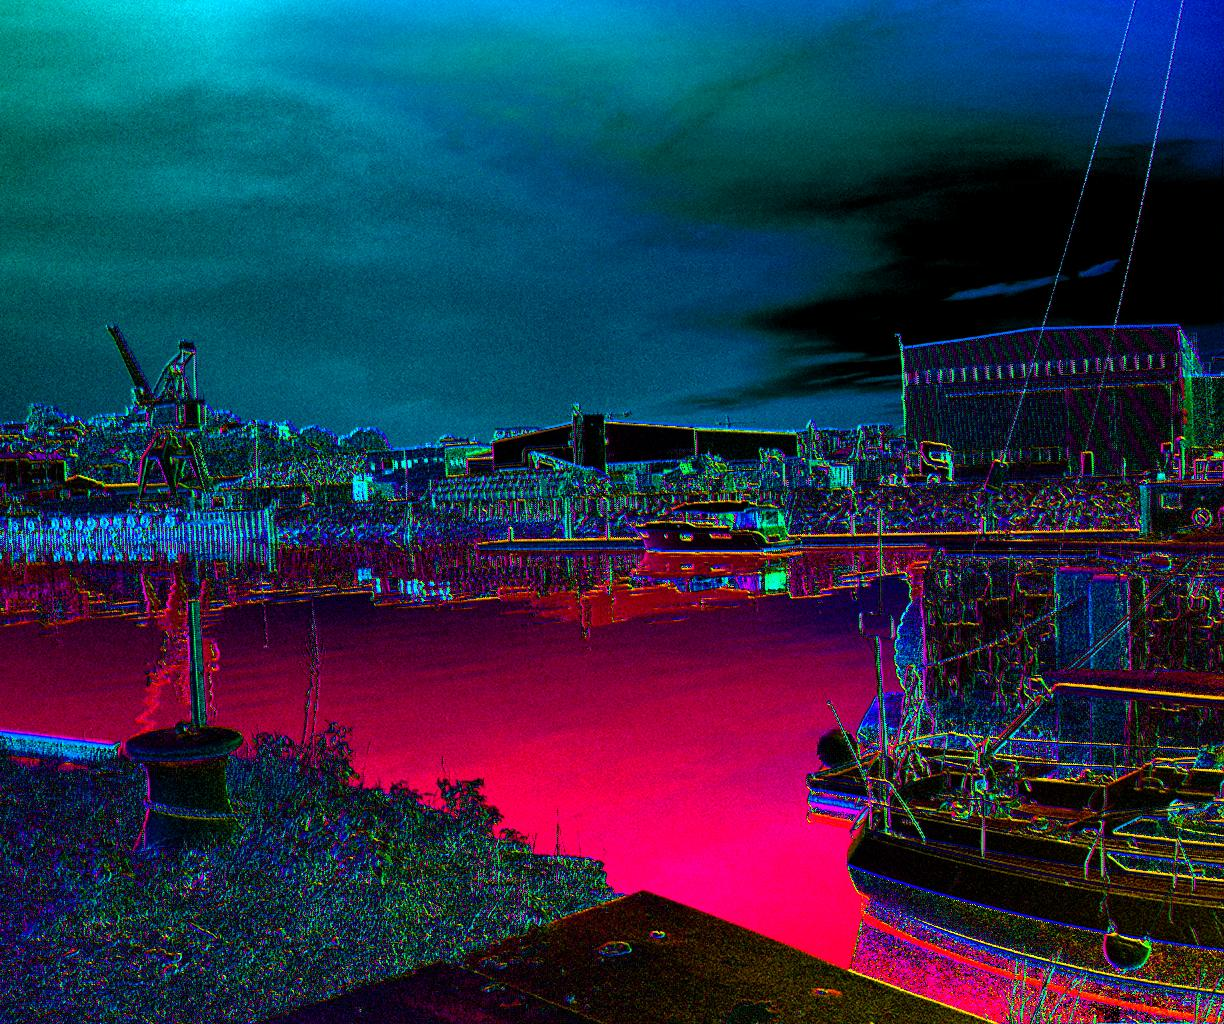
\includegraphics[width=.9\textwidth]{figures/pictures/aolp_left_124.jpeg}}
    \caption{Left image \#1984}
\end{figure}
\begin{figure}[H]
    \centering
    \subcaptionbox{Mean image.}{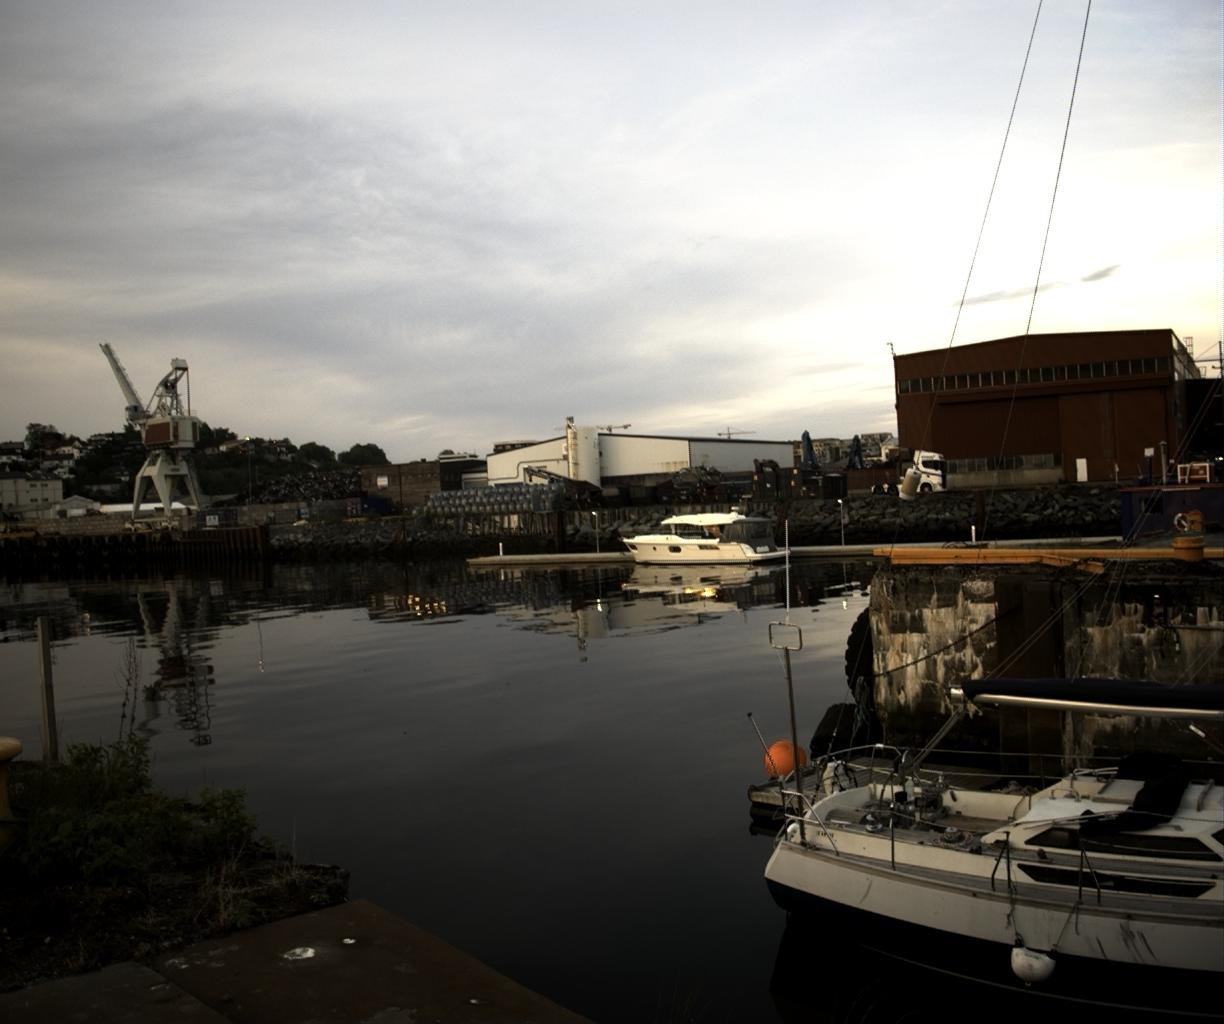
\includegraphics[width=.9\textwidth]{figures/pictures/regular_right_124.jpeg}}
    \subcaptionbox{HSV visualization.}{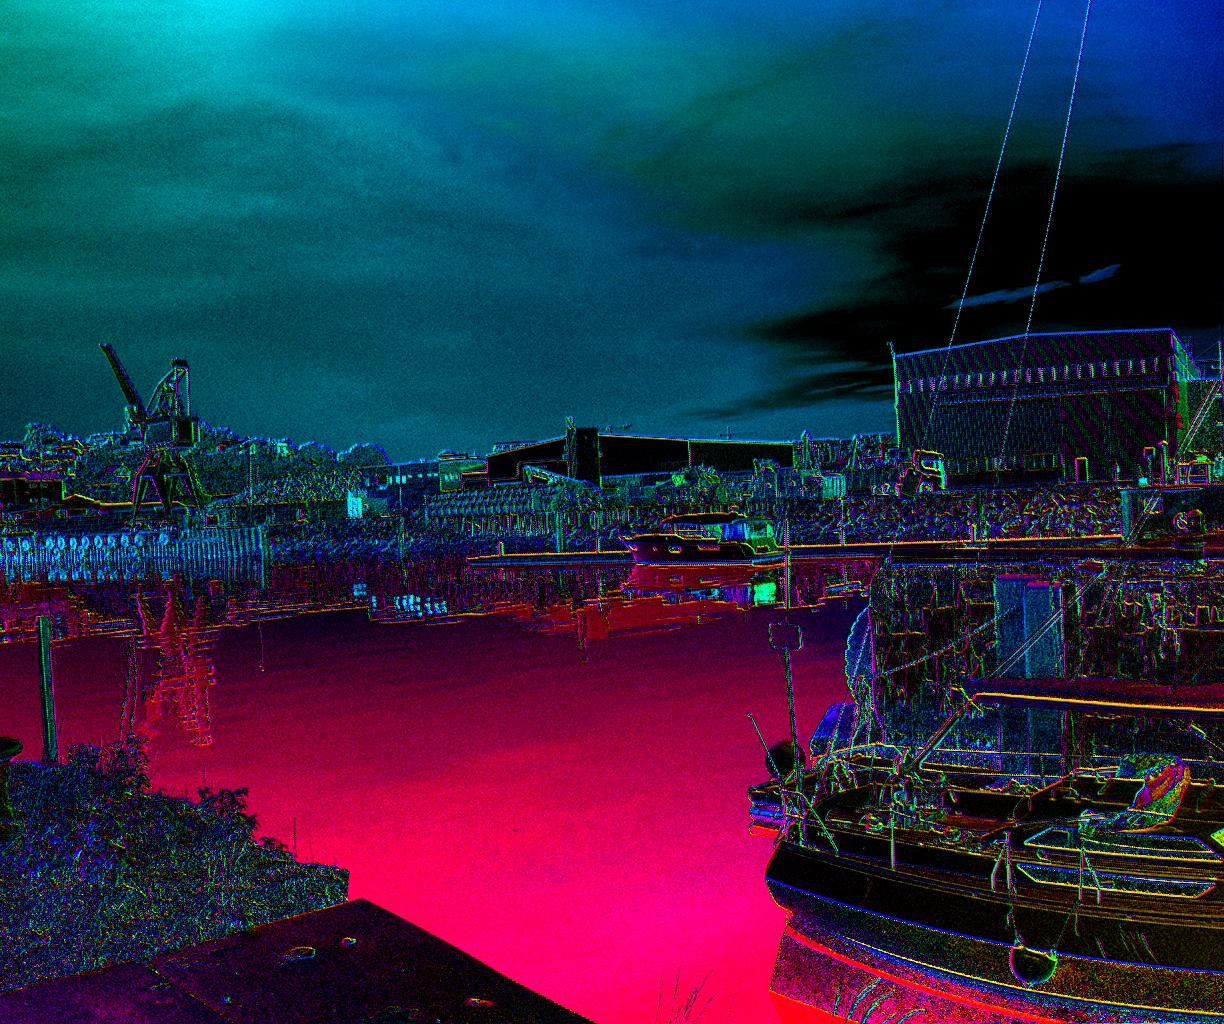
\includegraphics[width=.9\textwidth]{figures/pictures/aolp_right_124.jpeg}}
    \caption{Right image \#1984}
    \label{fig:picture_1984}
\end{figure}


\subsection{HSV}
Another color representation that is relevant in this \master is \gls{hsv}.
This format is what is usually used when selecting color in a color picker.
A usefull property of this format is that it can be used to easily visualize